\chapter{Proof of Work and Nakamoto Consensus}
Still it is note worthy to remember the two keywords for blockchains, decentralization, and trust. What we have discussed so far was that blockchain data structure enables a tamper-evident and tamper-resistant ledger but only a single party has the privilege to write into the ledger. We saw that this data structure has trust built into it. In this chapter we will go through the idea of decentralization and we will see that how bitcoin deals with decentralization via the Nakamoto consensus protocol.

\section{Decentralized Blockchain \& Nakamoto consensus}
We saw the idea of signature in the previous chapter. The identity of the signer is called the public key, in blockchain or Bitcoin terminology is simply called the address. In a Bitcoin wallet, the address simply reports the public key of the wallet. There is also a secret key corresponding to each public key. Giving away the secret key would be tantamount to giving away access to be able to let other people sign for you.\\\\
A coin has a unique identity that is linked to its owner. The owner is the person who received the coin in the last transfer transaction, which can be traced back to the original coin creation transaction or the Genesis block. In blockchains, some special people have the authority to create new coins. We will discuss who they are, how they got this power, and what are the principles and rules of coin creation in blockchains. This is related to the field of tokenomics, which studies the design and economics of tokens.\\\\
A signature can also be on a block itself.  If several people are writing to a database, then it may make sense to know who has signed it and who has entered the data. This data structure, or ledger, can be updated by a fixed and known group of parties who may not fully trust each other. They have a common interest in maintaining the ledger, but they need to follow certain rules to add new blocks to it. This could be a consortium. \\\\
Unlike some blockchains that limit the number of participants, Bitcoin is open and unlimited. Anyone can create as many identities as they want by generating public and private keys. Bitcoin is a free and decentralized system.

\subsection{Distributed consensus}
 When different people can update the ledger, who keeps track of all the changes? One way is to have everyone store the whole ledger, but this is very inefficient and costly. We will see how we can relax this assumption and make the system more scalable. They follow a protocol that lets them check and verify each other’s blocks. This is how they ensure the ledger’s integrity and security. Consensus or agreement is at the heart of trust.\\\\
Byzantine fault tolerance (BFT) is a property of a distributed system that allows it to reach a consensus among its components, even if some of them are faulty or malicious. BFT is important for ensuring the reliability and security of a distributed system, especially in scenarios where there is no central authority or trust among the participants. BFT is also relevant for blockchain systems, which are distributed networks that store and process transactions without relying on a central authority. Blockchain systems use consensus protocols to ensure that all nodes in the network agree on the same state of the ledger, despite the presence of faulty or malicious nodes.  You could use one of these BFT protocols to come up with an agreement among the participants on a block.\\\\
Bitcoin consensus protocol is so different from BFT protocols in some ways:
\begin{itemize}
    \item It's decentralized truly in the sense of permissionless.
    \item It makes less pessimistic network assumptions.
\end{itemize}
Now there will be a question that  \textbf{how do people come to consensus?}\\\\
Since in the case of Bitcoin, one can have several identities,  voting can not be an answer like it is for democracy. We need a way to have a consensus without voting. This was somehow assumed impossible before Nakamoto.
\subsection{Network Assumptions}
People in a consensus need to communicate with each other, in other words, we need a network among the participants.
Bitcoin assumptions for this concept are as follows:
\begin{itemize}
    \item Any node can broadcast to all nodes into the network and it's a fully connected network.
    \item Every broadcast message reaches every node albeit with some delay which is about 10 minutes for Bitcoin. 
\end{itemize}
These concepts and ideas will be discussed more in future chapters.

\subsection{Leader election: Oracle}
One way to quickly decentralize is to elect a leader. The leader's job is to put the block together and put it out for everybody to share. This sharing the block and creating it is called proposer, and this leader is said to be a proposal. Adding a new block to the ledger is a special role that requires some rules and restrictions. Otherwise, there would be too much conflict and confusion among the nodes. They need to agree on the same ledger state. A proposal is simply identified with a public key and not with an IP address or network (node).\\\\
The ledger is updated in regular intervals, called rounds. Blocks are not created randomly or too frequently (e.g. every second). For instance, in Bitcoin, the protocol specifies that a new block is added every 10 minutes. A node creates a new block by collecting all the new and valid transactions that it has seen on the network, and that are not already in previous blocks. This block is the node’s proposal for the next ledger state.\\\\
A transaction is valid if it meets two criteria:
\begin{enumerate}
    \item The sender of the coin must have owned the coin in a previous block in the ledger
    \item The sender must not have spent the coin twice in different transactions. This ensures that the coin is not duplicated or forged.
\end{enumerate}
At a glance here are the 4 main activities that a proposal does:
\begin{enumerate}
    \item constitutes a block with transactions
    \item validates transactions
    \item includes a hash pointer to the previous block
    \item signs the block
\end{enumerate}
A malicious proposer could try to cheat by signing a block when it was not their turn, or by inserting fake or invalid transactions in the block. However, this can be detected and prevented by the other nodes, who can verify the signature and the transactions. The proposer cannot fool the system by being dishonest or lazy. Everyone can verify the validity of transactions by using the ledger, which is a chain of blocks. Each block has a Merkle root that preserves the order of the transactions in the block. The ledger gives a complete history of all transactions ever made and allows anyone to track the current state of the coins and their owners. This is how validation is done.\\\\
Two kinds of messages are broadcasted in the network: transactions and proposals. Transactions are sent by anyone who wants to transfer coins, and they are stored in a temporary memory pool by the nodes. Proposals are created by special nodes who have the right to make new blocks, and they contain some transactions from the memory pool. The proposer can choose which transactions to include in the block, as long as the block size is one megabyte.\\\\
\subsection{Satoshi}
A satoshi is the smallest unit of a bitcoin, equivalent to 0.00000001 BTC. There are 100 million satoshi in one bitcoin.
\section{Proof of Work}
The method to elect a proposer that Bitcoin shows here in general is called proof of work. The goal of the competition is to select one of the participants to be the proposer. The competition proceeds like this.  Proof of work requires miners to solve complex mathematical problems using their computing power, which consumes a lot of energy. The problems are hard to solve but easy to verify, and the probability of finding a solution is proportional to the amount of work done. The first miner who finds a valid solution gets to create a new block of transactions and receive a reward in Bitcoin. The new block is then broadcast to the rest of the network and added to the chain of previous blocks, forming the blockchain.\\\\
The mathematical problem is a hash puzzle. Hash puzzles are a game in which one tries to find a nonce (an integer) such that 
\begin{align*}
    H(nonce, data) < T
\end{align*}
where T is the target difficulty level. If you can find a nonce, that's the proof of what is work here. We include nonce inside the block. The threshold is chosen such that a block is mined successfully on average once in 10 minutes.\\
The process of searching for a nonce that solves the hash puzzle is called mining.
\subsection*{Properties of Proof of Work}
\begin{enumerate}
    \item Random miner selected at each time
    \item Independent randomness across time and miners
    \item Probability of successful mining proportional to the fraction of total hash power
    \item Sybil resistance
    \item Spam resistance
    \item Tamper proof – even by the proposer!
\end{enumerate}
The chance of winning is proportional to how much hash power this miner brings to the competition. Hash power relates to the number of hashes I can try per second, which is directly proportional to how much GPUs energy I can bring.\\\\
Sybil resistance is the ability of a system to prevent or deter malicious actors from creating multiple fake identities or nodes to manipulate or attack the system. For example, in a peer-to-peer network, a sybil attacker could create many fake nodes to isolate, censor, or deceive honest nodes, or to gain more influence or voting power.
\section{Forks and Longest Chain Protocol}
 Forks and the longest chain rule are related to how the Bitcoin network reaches a consensus on the state of the ledger, which is a chain of blocks that contains all the transactions ever made.\\\\
A fork is a situation where there are two or more competing versions of the ledger, each with a different block at the end. A fork can happen when two miners find a valid block at the same time, or when some nodes do not receive or accept a new block. A fork can also be caused by malicious nodes who try to create fake or invalid blocks.
\begin{center}
    \begin{figure}[h!]
        \centering
        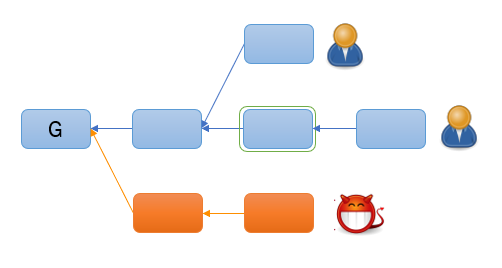
\includegraphics[width=0.6\linewidth]{Fig/03/F1}
        \caption{Forks in Blockchain}
        \label{fig:f1}
    \end{figure}
\end{center}
The longest chain rule is a way of resolving forks and choosing the valid version of the ledger. The longest chain rule states that the nodes should always follow and extend the chain of blocks that has the most accumulated proof-of-work, which is a measure of how much energy and effort was spent to create the blocks. The longest chain rule ensures that the majority of the network agrees on the same ledger and that any forked or orphaned blocks are discarded.
\begin{center}
    \begin{figure}[h!]
        \centering
        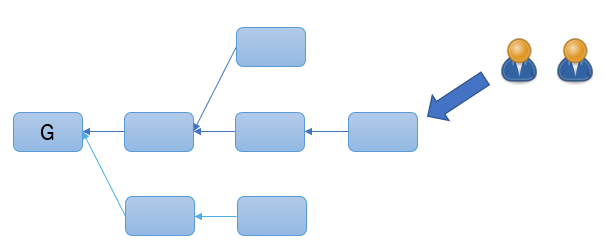
\includegraphics[width=0.6\linewidth]{Fig/03/F2}
        \caption{The longest chain rule}
        \label{fig:f2}
    \end{figure}
\end{center}


\section{Adversarial users}
The preceding description outlines the fundamental elements of the Nakamoto consensus protocol, with additional details to be covered in the forthcoming chapter. It is crucial for all users to strictly adhere to the protocol's guidelines. However, in real-world scenarios, there might be some users who deviate from the protocol, and these individuals are known as adversarial users or malicious users.\\\\
The primary objective of adversarial parties is to disrupt the system in any way possible. One particular attack they may employ to undermine the append-only property of the ledger is referred to as the \textbf{private attack}.\\\\
In the private attack scenario, the adversarial users engage in mining new blocks, but they refrain from broadcasting these blocks to the network. This secretive approach allows them to create an alternative chain, or "fork," in the blockchain that remains hidden from honest users. While the adversarial users continue to mine privately, honest users carry on with their mining activities, unaware of the existence of the private blocks.\\\\
Due to the inherent randomness in the mining process, the adversarial users might get lucky and quickly build a few private blocks in succession, let's say five blocks. Meanwhile, the honest users, during the same period, mine only three blocks on the public blockchain.\\\\
In this situation, the private (adversarial) chain becomes longer than the public (honest) chain because it has five blocks compared to the honest chain's three. Now, the adversarial users release their private chain to all other users, revealing the blocks they kept hidden.\\\\
As per the Nakamoto consensus protocol's longest-chain rule, honest users must adopt the chain with the greatest length. Since the private chain is now longer than the public chain, all honest users are compelled to give up their chain and switch to the adversarial chain. As a result, the last three blocks, which were part of the honest chain, are effectively erased from the ledger.\\\\
This action of adopting the longer chain effectively invalidates the transactions contained in the last three blocks of the honest chain, allowing the adversarial users to carry out a double-spending attack. By creating a longer chain with more proof-of-work, the adversarial users successfully overwrite the transaction history on the blockchain, causing disruption and undermining the append-only property of the ledger. This highlights the importance of consensus mechanisms in preventing such attacks and maintaining the integrity and security of decentralized ledgers.\\\\
Figure \ref{fig:f3} illustrates the fork in the blockchain resulting from a private attack:
\begin{enumerate}
    \item \textbf{Scenario:} \\A group of malicious users launches a private attack on the blockchain system.
    \item \textbf{Fork in the Blockchain:} \\The attack causes a fork in the blockchain, resulting in two competing chains of blocks.
    \item \textbf{Block Representation:} 
    \begin{itemize}
        \item Dashed blocks: These represent the privately held blocks generated by the adversarial users.
        \item Solid blocks: These represent the publicly visible blocks mined by honest users and part of the main blockchain.
    \end{itemize}
    \item \textbf{Private vs. Public Chain:}
     \begin{itemize}
        \item Private Chain: Comprises the dashed blocks, which remain hidden from the public network.
        \item Public Chain: Consists of solid blocks and is the main blockchain known to honest users.
     \end{itemize}
    \item \textbf{Objective:} \\The adversarial users aim to create a longer private chain compared to the public chain by exploiting the longest-chain rule in the Nakamoto consensus protocol.
    \item \textbf{Revealing the Private Chain:}\\Once the malicious users perceive that their private chain is longer, they reveal it to the entire network.
    \item \textbf{Switching to the Longer Chain:} \\Following the longest-chain rule, honest users must adopt the longer chain, abandoning the public chain they were initially working on.
    \item \textbf{Impact on the Ledger:}\\The switch to the adversarial chain effectively invalidates the transactions contained in the blocks of the public chain that are no longer part of the main blockchain.
\end{enumerate}
\begin{center}
    \begin{figure}[h!]
        \centering
        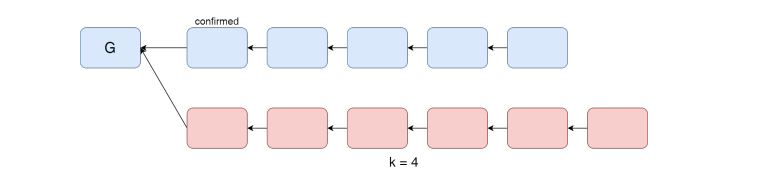
\includegraphics[width=0.6\linewidth]{Fig/03/F3}
        \caption{An Illustration of the private attack}
        \label{fig:f3}
    \end{figure}
\end{center}
This private attack undermines the integrity of the blockchain and demonstrates the significance of robust consensus mechanisms in preventing such disruptions and maintaining the security of decentralized ledgers.\\\\
The successful execution of private attacks can severely undermine trust in the blockchain system. One particularly impactful demonstration of this is the double-spend action enabled by the private attack. Let's explore this scenario using Figure \ref{fig:f4}:
\begin{enumerate}
    \item \textbf{The Initial Transaction:} A transaction ($tx$) is embedded in a block $B$. For instance, let's assume the transaction involves the payment of seven Bitcoins to Tesla, which has recently announced plans to accept Bitcoins for their cars.
    \item \textbf{Confirmation of the Transaction:} Upon seeing the transaction (tx) embedded in a block on the longest chain, Tesla confirms the transaction and releases the car to the source of the transaction. This action "confirms" or completes the transaction ($tx$) based on the longest chain, which Tesla considers valid.
    \item \textbf{Launching the Private Attack:} After the transaction ($tx$) has been confirmed, an adversary observing this development decides to launch a private attack. The adversary releases two or more blocks it had been secretly mining in private.
    \item \textbf{Impact of the Private Attack:} As a result of the private attack, the block $B$ containing the confirmed transaction ($tx$) is no longer part of the longest chain. Consequently, the transaction ($tx$) is no longer included in the ledger maintained by the network's participants.
    \item \textbf{Double-Spending Opportunity:} Now that the transaction ($tx$) has been removed from the ledger, the source of the transaction is free to double-spend the seven Bitcoins. This means they can use the same seven Bitcoins to initiate another transaction, effectively spending them twice.
    \item \textbf{Trust Demolished:} The successful double-spending attack seriously undermines the trust embodied by the blockchain system. It compromises the integrity of the ledger and erodes confidence in the security of the network.
\end{enumerate}
One way to address this vulnerability is by delaying the confirmation of transactions. By waiting for more blocks to be added to the chain after the transaction is initially embedded, the likelihood of a successful double-spending attack through a private attack is reduced. This delay allows the network to have more confidence in the validity of transactions before confirming them, enhancing the security and trustworthiness of the blockchain system.

\begin{center}
    \begin{figure}[h!]
        \centering
        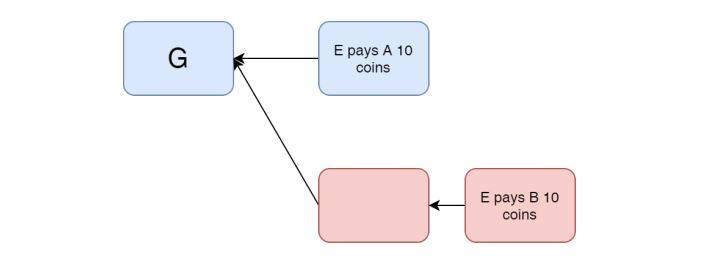
\includegraphics[width=0.6\linewidth]{Fig/03/F4}
        \caption{An Illustration of the double spend attack.}
        \label{fig:f4}
    \end{figure}
\end{center}


\section{The $k$-deep Confirmation Rule}
In the Nakamoto consensus protocol, occasional changes at the end of the ledger are impossible to avoid. These changes can be made by adversarial or by network delays.\\\\
Malicious users can collaborate and launch private attacks, as discussed earlier. By creating a longer chain in secret and releasing it to the public network, they can rewrite the last block of the ledger. This undermines the integrity of the ledger and poses a significant challenge to maintaining trust in the blockchain system.\\\\
Even without adversarial users, forks can occur in the blockchain due to network delays. When multiple blocks are mined simultaneously, they can propagate through the network at different speeds, leading to temporary forks. Honest users may work on different branches of the blockchain, resulting in competing chains.\\\\
Forks introduce the possibility of the longest-chain switching. As honest users continue mining and adding blocks to their respective branches, one of the branches might eventually become longer, leading to a shift in the longest-chain rule. When this happens, the blockchain system must adapt to the new longest chain, resulting in a rewriting of the last portion of the ledger.\\\\
Indeed, the solution to address the issue of occasional changes at the end of the ledger in the Nakamoto consensus protocol is simple and intuitive. By treating a block as confirmed only if it is buried deep enough under other blocks, the blockchain system can enhance its resilience against forks and ensure the immutability of the ledger. Here's a breakdown of the solution:
\begin{enumerate}
    \item \textbf{Confirmation Depth:} \\Users should consider a block as confirmed only if it is buried deep enough under a certain number of subsequent blocks. Let's denote this number as "k."
    \item \textbf{Consequences of Confirmation:}\\Confirming a block, say block B, means that the portion of the ledger up to that block is now considered immutable and secure. This implies that all transactions contained in the blocks preceding B are considered final and trustworthy.
    \item \textbf{Delayed Confirmation:}\\The solution suggests that it is not advisable to confirm very recent blocks immediately. New blocks are vulnerable to being overwritten due to forks in the blockchain. By delaying the confirmation of recent blocks, the system allows more time for the network to converge to a single valid chain.
    \item \textbf{Protection Against Forks:}\\By requiring a minimum depth of k blocks to confirm a specific block, the system provides protection against forks. Blocks that are not part of the longest chain, and therefore part of competing forks, will not be confirmed until a sufficient number of additional blocks are added to the chain, making it less likely for the confirmation to switch between forks.
    \item \textbf{Increasing Security Over Time:}\\As more blocks are added to the blockchain and the depth of confirmations increases, the security and finality of transactions improve. Deeper confirmations provide greater confidence that the ledger's history is unchangeable.
\end{enumerate}
This approach aligns with the practical behavior observed in many blockchain systems, where users and applications typically wait for a certain number of block confirmations before considering a transaction as fully settled. The higher the confirmation depth (larger k value), the more secure and reliable the transaction becomes.\\\\
By implementing this simple confirmation mechanism, blockchain systems can maintain the integrity of the ledger and safeguard against the potential disruptions caused by forks and private attacks, contributing to a more robust and trustworthy decentralized network.\\\\
The k-deep confirmation rule, as described earlier, is based on the belief that any changes in the longest chain will typically occur towards the end of the chain. The prefix of the longest chain at a specific time t, obtained by dropping the last k blocks, will continue to remain a prefix of the longest chain at future times as well. It is essential to note that this belief holds for most practical scenarios, but it is not guaranteed with absolute certainty for any finite value of k.\\\\
Certain conditions, such as adversarial users investing in significant computing power, disrupting block communication among honest users, or having an extraordinary stroke of luck, can potentially overturn a deeply buried block. However, as the value of k increases, the likelihood of such events happening diminishes significantly.\\\\
Chapter 6 demonstrates that the probability of such events decreases exponentially with k, under the assumption that the honest miners control a majority of the total hash power (i.e., more than 50\%). This assumption is critical in the Nakamoto consensus protocol, as it ensures that the honest miners collectively have more computational power than adversarial users, making it more improbable for adversarial users to consistently outpace the honest chain in mining blocks.\\\\
In summary, the k-deep confirmation rule, although not entirely foolproof, provides a practical and effective approach to enhance the security and reliability of the blockchain system. By requiring a certain depth of confirmations (larger k value) before considering a block as truly confirmed, the system minimizes the risk of chain reorganizations due to forks and private attacks. The larger the value of k, the lower the likelihood of such disruptive events happening, reinforcing the blockchain's robustness when honest miners have a majority of the hash power.\\\\
\section{Variable mining difficulty}
In PoW blockchains, adapting to the vast variation in mining power is essential for maintaining stability and security. One way to achieve this is through a difficulty adjustment algorithm. In the case of Bitcoin, the following three core ideas are used in its difficulty adjustment algorithm:\\
\begin{itemize}
    \item \textbf{(a) Varying the Difficulty Target: }The difficulty target for block mining is adjusted based on the average inter-block time from the previous epoch, which consists of 2016 blocks. If the average time is greater than the desired inter-block time (e.g., 10 minutes), the difficulty is reduced to make mining easier. Conversely, if the average time is less than the target, the difficulty is increased to make mining harder.
    \item \textbf{(b) Using the Heaviest Chain Rule: }Instead of considering the longest chain, the blockchain system determines the valid chain based on the total sum of block difficulties. The chain with the most accumulated proof-of-work (highest difficulty) is considered the heaviest chain and is used to determine the valid ledger.
    \item \textbf{(c) Mild Difficulty Adjustment: }The difficulty is adjusted only mildly at the end of each epoch, and the adjustment is bounded by a factor of 4. This prevents abrupt and drastic changes in the difficulty, ensuring a smoother transition during different mining periods.
\end{itemize}
While this algorithm may seem straightforward, simpler approaches can lead to dangerous security vulnerabilities. For example, using only the heaviest chain rule (b) and allowing miners to choose their difficulty can create significant problems.\\\\
An initial analysis might suggest that the heaviest chain rule does not provide an advantage for manipulating difficulty. However, this lack of advantage only holds in expectation, and extremely difficult adversarial blocks can introduce high variance, thwarting confirmation rules that confirm deeply embedded blocks with non-negligible probabilities proportional to the attacker's mining power\cite{reference1}.\\\\
For instance, suppose honest miners adopt the initial mining difficulty defined in the genesis block, with an expected inter-block time of 10 minutes (using 10 minutes as the unit of time). The difficulty unit is defined as the time it takes to mine an honest chain with k blocks. If the adversarial mining power is half of the honest mining power (or 1/3 of total mining power), the adversary can mine a single block as difficult as $k$ honest blocks within k units of time. The adversarial mining process follows a \textbf{Poisson} point process with a rate of 1/2k, and the number of adversarial blocks mined in $k$ units of time follows a Poisson distribution Poiss(1/2).\\\\
Hence the success probability of this attack would be:\\
\begin{equation*}
    P(\text{attack succeeds}) = P(\text{Poiss}(1/2) \geq 1) = 1 - e^{-1/2} \approx 39.3\%
\end{equation*}
which is a constant independent of $k$, therefore any $k$-deep confirmation rule will fail.\\\\
Consider a more detailed difficulty adjustment rule involving only (a) and (b), where the adversary can perform a difficulty-raising attack. The attack exploits the ability to create an epoch with extremely close-together timestamps, causing the difficulty adjustment rule to set the difficulty significantly higher for the next epoch. The attacker then utilizes the high variance in mining to execute the attack. Here's a description of this attack:
\begin{enumerate}
    \item \textbf{Adversarial Timestamps:} \\The adversary can manipulate timestamps in their private blocks, allowing them to create an epoch with timestamps that are extremely close together.
    \item \textbf{Difficulty Setting:}\\The difficulty adjustment rule (a) calculates the difficulty for the next epoch based on the average inter-block time from the previous epoch. If the timestamps in the adversary's private blocks indicate an extremely fast block generation rate, the difficulty for the next epoch will be set very high.
    \item \textbf{Difficulty-Raising Attack:}\\Let $B$ be the first block of the second epoch in the adversary's private chain, with difficulty $X$ . The chain difficulty of block $B$ is $2016 + X$, as it includes the difficulty of the previous $2016$ blocks.
    \item \textbf{Honest Chain Mining Time:}\\Mining an honest chain with chain difficulty $2016 + X$, on average, takes $2016 + X$ units of time.
    \item \textbf{Attack Preparation Time:}\\Considering the same adversary, it takes, on average, $4032$ units of time for them to complete the first epoch in their private chain.
    \item \textbf{Attack Execution:}\\To succeed in the attack, the adversary needs to mine block $B$ within $X − 2016$ units of time, which happens with a probability:\begin{equation*}
        P(\text{attack succeeds}) = P(\text{Poiss}\left(\frac{X-2016}{2X}\right) \geq 1) = 1 - e^{-(X-2016)/2X} \approx 1 - e^{-1/2} \approx 39.3\%
    \end{equation*}
    
\end{enumerate}
The attack's success probability is approximately $39.3\%$. If the adversary can accomplish this, they can create a difficulty spike for the next epoch, making it exceedingly difficult for honest miners to keep up with the fast mining rate. This high variance in mining can then be exploited by the attacker, allowing them to perform reorganizations, invalidate deeply embedded blocks, and potentially double-spend.\\\\
This difficulty-raising attack highlights the importance of a careful and sophisticated difficulty adjustment algorithm in PoW blockchains. The Bitcoin difficulty adjustment algorithm takes into account a combination of factors, such as average inter-block time, to prevent such attacks and maintain a stable and secure block generation rate over time. By carefully adjusting the difficulty at regular intervals and avoiding abrupt changes, the system can mitigate the risks associated with extreme variations in mining power and ensure the resilience of the blockchain network.\\\\
Correct, if $X >> 2016$, the success probability of the difficulty-raising attack remains significant, and it becomes more challenging to rely solely on a $k$-deep confirmation rule. This complex attack, which is only thwarted by the full protocol employing (a), (b), and (c) together, highlights the importance of the comprehensive Bitcoin difficulty adjustment algorithm. Let's formally describe the Bitcoin difficulty adjustment algorithm:\\\\
Consider a chain of $v$ blocks with timestamps $(r_1, \ldots, r_v)$. The Bitcoin difficulty adjustment algorithm uses the following fixed parameters:

\begin{itemize}
    \item $\tau$ (set to 4 in Bitcoin): The factor by which the difficulty is allowed to be adjusted mildly every epoch.
    \item $\Phi$ (set to $2016$ in Bitcoin): The length of an epoch in the number of blocks.
    \item $\Lambda_0$ (set to 2 weeks in Bitcoin): The expected duration of an epoch.
\end{itemize}

The difficulty adjustment algorithm aims to keep the average inter-block time close to the target block time (e.g., 10 minutes for Bitcoin) over the long term.\\\\
The algorithm operates as follows:

\begin{enumerate}
    \item Calculate the Time Difference:
    \begin{align*}
        D &= r_v - r_1
    \end{align*}
    
    \item Calculate the Expected Epoch Duration:
    \begin{align*}
        \Lambda &= \frac{\Lambda_0 \cdot D}{\Phi \cdot \tau}
    \end{align*}
    
    \item Adjust the Difficulty:
    \begin{align*}
        \text{If } D &< \frac{\Lambda}{2}, \text{ increase the difficulty threshold by a factor of }\tau \\
        \text{If } D &> 2 \Lambda, \text{ decrease the difficulty threshold by a factor of }\tau
    \end{align*}
    
    \item Keep the Difficulty within Bounds:
    \begin{align*}
        \text{Ensure that the difficulty adjustment is limited to a maximum increase or decrease of a factor of }\tau
    \end{align*}
\end{enumerate}
By adjusting the difficulty threshold based on the actual epoch duration and comparing it to the expected epoch duration, the algorithm maintains a relatively stable and predictable inter-block time over the course of a long duration. This prevents abrupt difficulty spikes or drops caused by significant changes in mining power and helps maintain the security and stability of the Bitcoin blockchain.\\\\
The full protocol, which employs (a), (b), and (c) together, effectively mitigates various types of attacks and ensures the integrity of the blockchain system, preventing malicious actors from manipulating the difficulty to their advantage.\\\\
The target calculation function D: Z$\ast$ → R is defined as
\begin{equation*}
    D(\epsilon) = T_0
\end{equation*}
\[
D(r_{1}, ..., r_{v})=\begin{cases}
    \frac{1}{\tau}T & \text{if} \frac{\Lambda}{\Lambda_0}T \textless \frac{1}{\tau}T \\
    \tau T & \text{if} \frac{\Lambda}{\Lambda_0}T  \textgreater \tau T\\
    \frac{\Lambda}{\Lambda_0}T & \text{otherwise}
\end{cases}
\]
where $T_0$ is the initial target as defined in the genesis block, and $\Phi'$, $\Lambda$, and $T$ correspond to the last block, duration, and target of the last completed epoch, respectively, i.e., $\Phi' = \Phi\left\lfloor\frac{v}{\Phi}\right\rfloor$, $\Lambda = r_{\Phi'} - r_{\Phi'-\Phi}$, and $T = D(r_1,\dots,r_{\Phi'-1})$. A full and beautiful analysis of the Bitcoin protocol is provided in~\cite{reference2}.

\begin{center}
    \begin{figure}[h!]
        \centering
        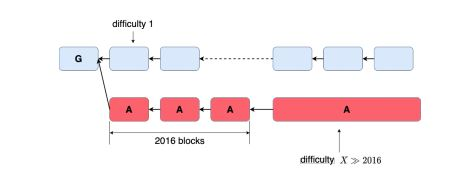
\includegraphics[width=0.6\linewidth]{Fig/03/F5}
        \caption{The difficulty rising attack. The adversary raises the difficulty to extremely high in the second epoch by faking timestamps.}
        \label{fig:f5}
    \end{figure}
\end{center}
\section{Bitcoin is Permissionless}
In the context of Bitcoin, participants have the freedom to generate multiple (secret key, public key) pairs for themselves, allowing them to create multiple identities. This feature is encouraged for privacy reasons, making Bitcoin a permissionless system. However, creating multiple identities does not grant an individual more influence in the system. The actual representation and power in Bitcoin are determined by the computational (mining) power, which can only be increased through capital investment in hardware and resources. This property ensures that the system is resistant to Sybil attacks, where an adversary could gain an advantage by creating numerous fake identities.\\\\
The PoW mining process in Bitcoin serves multiple important purposes simultaneously:\\\\
\begin{itemize}
    \item \textbf{(a) Sybil-Resistance: }By tying mining power to computational resources and capital investment, Bitcoin prevents individuals from easily gaining control of the system through the creation of multiple identities.
    \item \textbf{(b) Randomized Block Proposer Election: }PoW mining introduces an element of randomness to the selection of the miner who gets to propose the next block. The probability of being chosen as the block proposer is proportional to the miner's computational power. This process ensures that block proposals are distributed across different miners, enhancing the decentralization of the network.
    \item \textbf{(c) Adjusting Inter-Block Duration:} As discussed earlier, the PoW difficulty adjustment algorithm regulates the inter-block time, maintaining a relatively stable and predictable block generation rate.
\end{itemize}
In contrast to Bitcoin's permissionless nature, some other blockchain designs implement external mechanisms to ensure that each entity has only a single key, creating a permissioned system. In such permissioned blockchains, separate mechanisms are used for achieving goals (b) and (c) mentioned above, while still maintaining Sybil-resistance through other means.\\\\
In subsequent chapters, we will explore some of these other blockchain designs and understand how they address different aspects of consensus, security, and decentralization. Each design may have its trade-offs and may be better suited for specific use cases depending on the requirements of the application.

\renewcommand{\bibname}{References}
\begin{thebibliography}{9}
    \bibitem{reference1} Lear Bahack. Theoretical Bitcoin attacks with less than half of the computational power (draft). \textit{arXiv preprint arXiv:1312.7013, 2013}
    \bibitem{reference2} Garay, J., Kiayias, A., \& Leonardos, N. (2020). Full analysis of Nakamoto consensus in bounded-delay networks. Cryptology ePrint Archive, Report 2020/277. \url{https://eprint.iacr.org/2020/277}
\end{thebibliography}